\documentclass[../../ASSD_TP1_G7.tex]{subfiles}
\begin{document}
\chapter*{Oscilador}
Se dise\~no un oscilador cuya salida sea cuadrada, de frecuencia variable y de duty cycle variable. Ambos parámetros capases de variar independientemente uno de otro.
\subsection*{Circuito implementado}
Para lograr la independencia en la variación de frecuencia y duty cycle, se propuso un circuito de dos bloques, uno encargado de la frecuencia y el otro del duty cycle.
\begin{figure}[H]
\centering
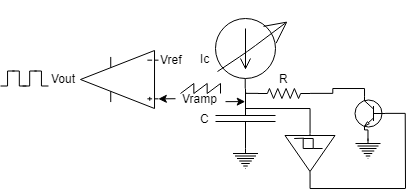
\includegraphics[width=0.5\textwidth]{figures/diagBloques.png}
\caption{Diagrama en bloques del circuito}
\end{figure}
\par El bloque correspondiente al control de la frecuencia es el de la fuente variable de corriente, el capacitor y el schmitt trigger. Como $i_c=\frac{d_v}{d_t}$, donde $i_c$ es la corriente en el capacitor, es constante debido a la fuente de corriente entonces la tension en el capacitor crece lienealmente en el tiempo,$V_c=t \frac{i_c}{C}$. Alcanzado la tension $V_{high}$ del schmitt trigger, su salida pasara a nivel alto y el transistor entrara en saturacion, descargando el capacitor. Cuando la tension el el capacitor alcance la tension $V_{low}$, la salida del schmitt trigger pasara a nivel bajo y la descarga del capacitor se detiene.
Variando $i_c$ se generan distintas pendientes de la rampa, a mayor pendiente mayor frecuencia. 
\par El bloque correspondiente al control del duty cycle, es el del comparador. Variando la tension de referencia($V_{ref} $), del comparador se logra el control del duty cycle. Cuando la tension en el capacitor supera a $V_{ref} $ la salida del comparador pasa a estado alto.
\subsubsection*{Implementación del modulo de control de frecuencia}
El modulo consta de dos partes:
\begin{itemize}
  \item Fuente variable de corriente
  \item Modulo para descargar el capacitor
\end{itemize}



\end{document}
